\section{Implementierung in \textit{C++}}
\label{sec:implementation}

Der folgende Quellcodeausschnitt zeigt eine Implementierung der direkten, diskreten Convolution
nach Summenformel \ref{eq:directConv}:

% Farben für Code definieren
\definecolor{codegreen}{rgb}{0,0.6,0}
\definecolor{codegray}{rgb}{0.5,0.5,0.5}
\definecolor{codepurple}{rgb}{0.58,0,0.82}
\definecolor{backcolour}{rgb}{0.95,0.95,0.92}

\lstset{
    language=C++,
    backgroundcolor=\color{backcolour},   
    commentstyle=\color{codegreen},
    keywordstyle=\color{blue},
    numberstyle=\tiny\color{codegray},
    stringstyle=\color{codepurple},
    basicstyle=\ttfamily\small,
    breakatwhitespace=false,         
    breaklines=true,                 
    captionpos=b,                    
    keepspaces=true,                 
    numbers=left,                    
    numbersep=5pt,                  
    showspaces=false,                
    showstringspaces=false,
    showtabs=false,                  
    tabsize=2
}

\lstinputlisting
[language=C++, linerange={20-38}, caption={Grundalgorithmus der Convolution im Zeitbereich},
label={lst:directConvolution}
]
{code/test/JuceTest/Source/convolution.cpp}

Als Parameter werden im Quellcode \ref{lst:directConvolution} zwei Listen, nämlich jeweils die Folgen
an normalisierten Abttaswerten des Eingangssignals und der Impulssantwort, übergeben.
Dadurch, dass die Beträge/Längen der Folgen bekannt sind, lässt sich in den Zeilen 5 bis einschl. 8
im Voraus die Länge der Ausgangssignalfolge nach $|y[n]| = |h[n]| + |x[n]| - 1$ berechnen und die Werte mit 0 initialisieren.
Schließlich wird die Formel \ref{eq:directConv} in Form der verschachtelten Schleife
in Zeilen 9 bis 16 umgesetzt. In manchen Schleifeniterationen kommt es dazu, dass der Index von $x[n - k]$
kleiner als null wird oder die Länge des Eingangssignals übersteigt. Diese Fälle werden in Zeile 11 geprüft und
ggf. wird die jeweilige Iteration der Schleife übersprungen.

Diese Vorgehensweise ist unter Kenntnis der diskreten Gleichung der Convolution \ref{eq:directConv}
leicht nachzuvollziehen, weil sie hier direkt in Code umgesetzt wird.
Es gibt aber hinsichtlich der Nutzung in der Praxis ein großes Problem, das durch die folgende Laufzeitmessung unterstrichen wird:

\begin{figure}[H]
    \centering
    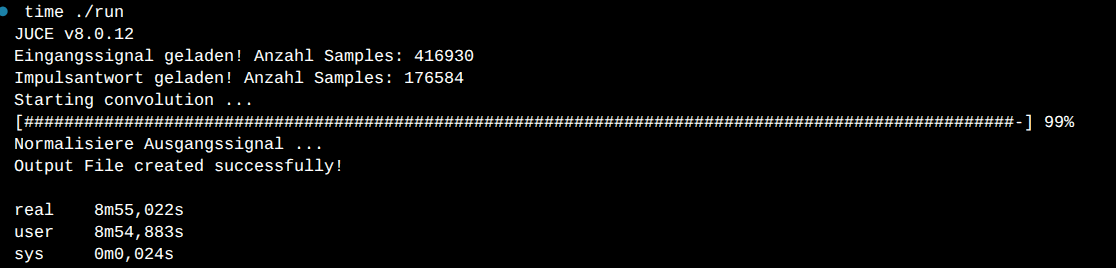
\includegraphics[width=1.0\textwidth]{graphic/img/chapterImpl/LfzDirekteFaltung.png}
    \caption{Laufzeitmessung des Algorithmus \ref{lst:directConvolution} unter Verwendung
    des Linux-Kommandos \textit{time}}
    \label{img:LfzMessungDirekteFaltung}
\end{figure}

Das Ergebnis der Messung, die in Abbildung \ref{img:LfzMessungDirekteFaltung} gezeigt wird,
bezieht sich auf die Convolution eines 10-sekündigen Gitarrensignals (416.960 Abtastungen) mit einer Impulsantwort von
5 Sekunden (176.584 Abtastungen). Ergebnis ist ein Halleffekt auf der Gitarre.
Wie an der Messung zu sehen ist, dauerte die Berechnung des 15-sekündigen Resultats fast ganze 9 Minuten an.
Diese Dauer ergibt in Anbetracht der zweifach verschachtelten Schleife und der Menge an Abtastwerten durchaus Sinn.
Schaut man sich im Quellcode \ref{lst:directConvolution} die Anzahl der Schleifendurchläufe, jew. von innerer und äußerer
Schleife an, dann ergibt sich folgende Laufzeitklasse:
\begin{equation}
\mathcal{O}(N \cdot M)
\label{eq:LfzDirekteFaltung}
\end{equation}
\textit{N} sei hierbei die Länge des Ausgangssignals und \textit{M} die Länge der Impulsantwort.
Dies ist kongruent zu der in der Sektion \ref{sec:runtime_analysis} gezeigten Laufzeitkomplexität.

Das entspricht speziell in diesem Experiment ausmultipliziert 104.805.076.176 Berechnungen, die der Prozessor also für ein
15-sekündiges Audiosignal ausführen muss.
Eine solche Laufzeit ist für den Gebrauch in der Praxis nicht hinnehmbar und der Grund, weshalb Berechnungen
der diskreten Convolution lange Zeit ausschließlich in der Forschung ihren Platz fanden \cite[Kap. 4]{lyons2011}.
